% This is the Reed College LaTeX thesis template. Most of the work
% for the document class was done by Sam Noble (SN), as well as this
% template. Later comments etc. by Ben Salzberg (BTS). Additional
% restructuring and APA support by Jess Youngberg (JY).
% Your comments and suggestions are more than welcome; please email
% them to cus@reed.edu
%
% See https://www.reed.edu/cis/help/LaTeX/index.html for help. There are a
% great bunch of help pages there, with notes on
% getting started, bibtex, etc. Go there and read it if you're not
% already familiar with LaTeX.
%
% Any line that starts with a percent symbol is a comment.
% They won't show up in the document, and are useful for notes
% to yourself and explaining commands.
% Commenting also removes a line from the document;
% very handy for troubleshooting problems. -BTS

% As far as I know, this follows the requirements laid out in
% the 2002-2003 Senior Handbook. Ask a librarian to check the
% document before binding. -SN

%%
%% Preamble
%%
% \documentclass{<something>} must begin each LaTeX document
\documentclass[12pt, oneside, openright]{byuthesis}


\title{Determining the significance of a consistent mode choice between activity-based models and agent-based microsimulation tools}
\author{Christopher Day}
\copyyear{2022}
\committeeMembers{Brigham Young, Chair

Karl G. Maeser

Harvey Fletcher}
\keywords{Four Step Model, Discrete Choice Model, Activity-based Model}
\degree{Master of Science}
\doctype{thesis}
\department{Department of Civil and Construction Engineering}



% End of CII addition
%%
%% End Preamble
%%
%

% Pandoc citation processing
\newlength{\cslhangindent}
\setlength{\cslhangindent}{1.5em}
\newlength{\csllabelwidth}
\setlength{\csllabelwidth}{3em}
\newlength{\cslentryspacingunit} % times entry-spacing
\setlength{\cslentryspacingunit}{\parskip}
% for Pandoc 2.8 to 2.10.1
\newenvironment{cslreferences}%
  {}%
  {\par}
% For Pandoc 2.11+
\newenvironment{CSLReferences}[2] % #1 hanging-ident, #2 entry spacing
 {% don't indent paragraphs
  \setlength{\parindent}{0pt}
  % turn on hanging indent if param 1 is 1
  \ifodd #1
  \let\oldpar\par
  \def\par{\hangindent=\cslhangindent\oldpar}
  \fi
  % set entry spacing
  \setlength{\parskip}{#2\cslentryspacingunit}
 }%
 {}
\usepackage{calc}
\newcommand{\CSLBlock}[1]{#1\hfill\break}
\newcommand{\CSLLeftMargin}[1]{\parbox[t]{\csllabelwidth}{#1}}
\newcommand{\CSLRightInline}[1]{\parbox[t]{\linewidth - \csllabelwidth}{#1}\break}
\newcommand{\CSLIndent}[1]{\hspace{\cslhangindent}#1}

\providecommand{\tightlist}{%
  \setlength{\itemsep}{0pt}\setlength{\parskip}{0pt}}

\usepackage{color}
\usepackage{fancyvrb}
\newcommand{\VerbBar}{|}
\newcommand{\VERB}{\Verb[commandchars=\\\{\}]}
\DefineVerbatimEnvironment{Highlighting}{Verbatim}{commandchars=\\\{\}}
% Add ',fontsize=\small' for more characters per line
\usepackage{framed}
\definecolor{shadecolor}{RGB}{248,248,248}
\newenvironment{Shaded}{\begin{snugshade}}{\end{snugshade}}
\newcommand{\AlertTok}[1]{\textcolor[rgb]{0.94,0.16,0.16}{#1}}
\newcommand{\AnnotationTok}[1]{\textcolor[rgb]{0.56,0.35,0.01}{\textbf{\textit{#1}}}}
\newcommand{\AttributeTok}[1]{\textcolor[rgb]{0.77,0.63,0.00}{#1}}
\newcommand{\BaseNTok}[1]{\textcolor[rgb]{0.00,0.00,0.81}{#1}}
\newcommand{\BuiltInTok}[1]{#1}
\newcommand{\CharTok}[1]{\textcolor[rgb]{0.31,0.60,0.02}{#1}}
\newcommand{\CommentTok}[1]{\textcolor[rgb]{0.56,0.35,0.01}{\textit{#1}}}
\newcommand{\CommentVarTok}[1]{\textcolor[rgb]{0.56,0.35,0.01}{\textbf{\textit{#1}}}}
\newcommand{\ConstantTok}[1]{\textcolor[rgb]{0.00,0.00,0.00}{#1}}
\newcommand{\ControlFlowTok}[1]{\textcolor[rgb]{0.13,0.29,0.53}{\textbf{#1}}}
\newcommand{\DataTypeTok}[1]{\textcolor[rgb]{0.13,0.29,0.53}{#1}}
\newcommand{\DecValTok}[1]{\textcolor[rgb]{0.00,0.00,0.81}{#1}}
\newcommand{\DocumentationTok}[1]{\textcolor[rgb]{0.56,0.35,0.01}{\textbf{\textit{#1}}}}
\newcommand{\ErrorTok}[1]{\textcolor[rgb]{0.64,0.00,0.00}{\textbf{#1}}}
\newcommand{\ExtensionTok}[1]{#1}
\newcommand{\FloatTok}[1]{\textcolor[rgb]{0.00,0.00,0.81}{#1}}
\newcommand{\FunctionTok}[1]{\textcolor[rgb]{0.00,0.00,0.00}{#1}}
\newcommand{\ImportTok}[1]{#1}
\newcommand{\InformationTok}[1]{\textcolor[rgb]{0.56,0.35,0.01}{\textbf{\textit{#1}}}}
\newcommand{\KeywordTok}[1]{\textcolor[rgb]{0.13,0.29,0.53}{\textbf{#1}}}
\newcommand{\NormalTok}[1]{#1}
\newcommand{\OperatorTok}[1]{\textcolor[rgb]{0.81,0.36,0.00}{\textbf{#1}}}
\newcommand{\OtherTok}[1]{\textcolor[rgb]{0.56,0.35,0.01}{#1}}
\newcommand{\PreprocessorTok}[1]{\textcolor[rgb]{0.56,0.35,0.01}{\textit{#1}}}
\newcommand{\RegionMarkerTok}[1]{#1}
\newcommand{\SpecialCharTok}[1]{\textcolor[rgb]{0.00,0.00,0.00}{#1}}
\newcommand{\SpecialStringTok}[1]{\textcolor[rgb]{0.31,0.60,0.02}{#1}}
\newcommand{\StringTok}[1]{\textcolor[rgb]{0.31,0.60,0.02}{#1}}
\newcommand{\VariableTok}[1]{\textcolor[rgb]{0.00,0.00,0.00}{#1}}
\newcommand{\VerbatimStringTok}[1]{\textcolor[rgb]{0.31,0.60,0.02}{#1}}
\newcommand{\WarningTok}[1]{\textcolor[rgb]{0.56,0.35,0.01}{\textbf{\textit{#1}}}}

\begin{document}

\begin{abstract}
This document describes the use of a new \LaTeX ~template for writing masters
theses at Brigham Young University. This was made necessary by the relative age
and complication of prior templates. Additionally, the new \texttt{cosmodown} R package
contains an implementation of this thesis in R markdown, with the help of the
\href{https://github.com/ismayc/thesisdown}{\texttt{thesisdown}} package.

The abstract of a thesis should describe the
motivation, objective, overall results, and central findings of the thesis.
It may have multiple paragraphs if necessary.
\end{abstract}


\makefrontmatter % this stuff will be roman-numbered
\thesisbody

\hypertarget{outline}{%
\chapter{Outline}\label{outline}}

Here is my outline for the entire thesis. Hopefully this will give me a rough idea of what to write about.

\begin{enumerate}
\def\labelenumi{\arabic{enumi}.}
\tightlist
\item
  Introduction \emph{(5pg)}
\end{enumerate}

\begin{verbatim}
a. First/Last mile transit
\end{verbatim}

\begin{enumerate}
\def\labelenumi{\arabic{enumi}.}
\setcounter{enumi}{1}
\tightlist
\item
  Literature Review \emph{(20-30pg)}
\end{enumerate}

\begin{verbatim}
a. Discus Mode Choice (4-step model, ABMs, microsimulations)
b. Discuss ActivitySim (modechoice)
c. Discuss MATSim (modechoice)
d. Discuss BEAM (modechoice)
e. Figure explaining tour type and first trip difference?
f. Variables showing path,person,location?
\end{verbatim}

\begin{enumerate}
\def\labelenumi{\arabic{enumi}.}
\setcounter{enumi}{2}
\tightlist
\item
  Methods
\end{enumerate}

\begin{verbatim}
a. What did we add to BEAM?
b. Algorithms
c. How did we make scenario?
d. What scenarios did we run? SLC + SL / Data & Calibration
e. What tests did we run? (path, person, location effects)
\end{verbatim}

\begin{enumerate}
\def\labelenumi{\arabic{enumi}.}
\setcounter{enumi}{3}
\tightlist
\item
  Results
\end{enumerate}

\begin{verbatim}
a. Describe tests and findings
\end{verbatim}

\begin{enumerate}
\def\labelenumi{\arabic{enumi}.}
\setcounter{enumi}{4}
\tightlist
\item
  Discussion
\end{enumerate}

\begin{verbatim}
a. What does it mean?
b. Limitations --> Future research recommendation
\end{verbatim}

\begin{enumerate}
\def\labelenumi{\arabic{enumi}.}
\setcounter{enumi}{5}
\tightlist
\item
  Conclusions
\end{enumerate}

\begin{verbatim}
a. Wider implications
b. First mile last mile
c. climate change lol
\end{verbatim}

\hypertarget{introduction}{%
\chapter{Introduction}\label{introduction}}

The basic outline for the literature review is as follows:

\begin{enumerate}
\def\labelenumi{\alph{enumi}.}
\tightlist
\item
  Mode choice in the Four step model
\item
  Mode Choice in Discrete Choice Modeling
\item
  Mode choice in Activity-based models
\item
  Mode choice in Activity-Sim
\item
  Mode choice in MATSim
\item
  Mode choice in BEAM
\item
  Mode choice difference between activity-based models and microsimulation tools
\item
  Importance of multiple variables in mode choice calculation
\end{enumerate}

\hypertarget{literature-review}{%
\chapter{Literature Review}\label{literature-review}}

Mode choice models are essential components in the transportation planning process. Key investment decisions along with other transportation decisions rely on the determination of individual mode choices within a population. Whether mode choice is estimated in a four step model, activity-based model, or an agent based model, its level of significance remains the same.

\hypertarget{lit1}{%
\section{Mode Choice in the Four Step Model}\label{lit1}}

The four step model (FSM) has been the primary tool in person travel demand modeling since its development (McNally 2000). Although travel is theorized to be derived from activity participation, the FSM focuses on modeling with trip-based not activity-based travel methods. The methodology presented in the FSM is mostly universal. The FSM can be divided up into two stages. The first defining the traveler and land use characteristics and the second where demand is loaded onto a transportation network and travel characteristics are determined (McNally 2000).

As its name suggests, the FSM includes four different steps: trip generation, trip distribution, mode choice, and route choice. In trip generation the magnitude of total trips is estimated and in trip distribution those trips are disbursed along different directions of travel. In mode and route choice, a multitude of variables are used to determine specifically how travel occurs.

Of the four steps in the FSM, mode choice in particular is a diverse, variable, and disaggregate step among different modeling applications. According to McNally (2000), mode choice is almost exclusively modeled on a disaggregate level within separate choice-based sampling. Choice probabilities are calculated on the individual trip level. McNally (2000) also mentions that with transit, carpooling vehicles, automobile tolls, and other new factors the mode choice algorithm can become extensive and difficult to determine. One common method used to estimate mode choice probabilities is a nested logit model (see Section \ref{lit3}). These mode choice models can reflect trip-maker characteristics as well as multiple performance variables (Ortuzar and G.Willumsen 1994; McNally 2000). Most applications of the FSM require multiple iterations of the mode choice and trip distribution steps in order to approximate formal convergence. Like with the nested logit model, discrete choice modeling has historically been the perferred method in estimating mode choice in the FSM as well as in other modeling applications.

\hypertarget{lit2}{%
\section{A Brief History of Mode Choice in Discrete Choice Models}\label{lit2}}

Various choice modeling systems have been used to accurately determine mode choices. The beginning of such analyses started with the developments of McFadden et al. (1973), who outlined a general procedure for modeling population choice behavior from distributions of individual decision rules. Before then, discrete choices were simply modeled using a random utility model (RUM) framework. The interpretation assumed that each individual carried their own utility function distribution and selected one randomly; according to Manski (2001), McFadden reinterpreted the random assignment of the utility functions across the population itself rather than the individual. This yielded an entirely new view of discrete choice modeling, and a more general version of the multinomial logit model (MNL) was introduced. This new MNL model, also called the conditional logit analysis, was the beginning of modern mode choice analysis. Goulias, Davis, and Bhat (2020) describe that McFadden's MNL model, the nested logit model, and the multinomial probit model (MNP) were the main engines in mode choice and most discrete choice analyses up through the 1990s.

Although the developments of McFadden are still in effect today, mode choice analysis has evolved greatly in the last few decades. Goulias, Davis, and Bhat (2020) explain that up through 2010, mixed multinomial logit (MMNL) models and multiple discrete-continuous (MDC) choice models were the main models in practice. In addition, Bhat (1995) estimated a disaggregate mode choice model to explain how new and updated services affected ridership and mode choice on intercity travel. His heteroscedastic extreme value model overcame the independence of irrelevant alternatives (IIA) property and allowed more flexibility among the alternatives than the nested logit model. Ben-Akiva, Mcfadden, et al. (2002) developed a hybrid choice model (HCM) that went beyond the standard RUM as it included latent variables, latent classes, and a flexible error structure. It implemented multiple facets of discrete choice modeling and more accurately represented the behaviors of the individuals. Pinjari et al. (2007) used a simultaneous mixed logit model to understand how commuters' mode choice is affected by the surrounding build environment.

According to Goulias, Davis, and Bhat (2020), from 2010 to 2015 joint models of data with mixed dependent variables arrived. Vij, Carrel, and Walker (2013), for example, used a behavioral mixtures model, composed of a latent class choice model (LCCM) and a continuous logit mixture model, to extrapolate unobserved modality styles and their effects on travel decisions. Paulssen et al. (2014) focused on improving the integrated choice and latent variable (ICLV) model of McFadden (1986) and Ben-Akiva, Walker, et al. (2002) by including a value system among the individuals. Overall, the general advancement within mode choice and discrete choice modeling is comprehensive across recent years. Similarly, the variability among mode choice analysis can specifically be seen within activity-based modeling.

\hypertarget{lit3}{%
\section{An Extensive Look into Mode Choice in Activity-Based Models}\label{lit3}}

A significant part of activity-based modeling is the mode choice decision within the model. Bhat and Koppelman (1999) stated that originally travel demand models used individual trips as the primary unit of analysis. In recent years though, there has been a shift toward activity-based travel demand modeling. According to Eluru et al. (2010), this shift has occurred due to improved understanding of activity-based travel, global climate concerns, and advances in microsimulation techniques. With this shift to activity-based travel modeling, FSMs have evolved immensely, and especially within the last decade (Hasnine and Nurul Habib 2021). A major maturing in activity scheduling, activity duration, activity generation, and location choice has occurred and resulted in advanced activity-based modeling. Although these components have evolved significantly, the mode choice decision has remained relatively simple and constant.

In general, the two types of mode choice models commonly applied in travel demand modeling are trip-based and tour-based models. Trip-based mode choice models select modes based on the characteristics of individual trips, independent of other existing trips. A tour is defined as a chain of trips that end in the same location as they start (John L. Bowman et al. 1999). Tour-based models are based on the characteristics of the trips' overarching tour, meaning trip modes are not independently calculated. Most activity-based models commonly implement the tour-based mode choice structure (Hasnine and Nurul Habib 2021).

In reality, the most common use of the tour-based mode choice model is the ``simplified tour-based'' mode choice model. The simplified tour-based model has been used in a variety of studies (Arentze and Timmermans 2000; J. L. Bowman and Ben-Akiva 2001; Pendyala et al. 1997). This simplified model hinges on trip-based mode choice where a single mode is used to define the entire tour opposed to a string of possible mode option combinations. For example, a simplified tour-based mode choice would define the tour-mode as ``public transit'' whereas a true tour-based model would define the tour-mode as ``public transit - ride hail - public transit''. Simplified tour-based models overlooks mobility attributes as well as the dynamics that exist between trips on a tour (Hasnine and Nurul Habib 2021).

There have been many attempts during the last few decades to include trip and tour based mode choice models into activity-based models.As a way to better understand the diversity that exists with tour-based mode choice in activity-based models, Hasnine and Nurul Habib (2021) conducted research on a variety of activity-based models from the years 1995 to 2020 and found that seven specific mode choice analyses have been used. All seven techniques are framed about the tour-based methodology further reinforcing the knowledge that ``the tour-based approach is the most relevant to the activity-based modelling framework'' (Hasnine and Nurul Habib 2021). These seven categories are further discussed in the following subsections.

\hypertarget{simplified-main-tour-model}{%
\subsection{Simplified main tour model}\label{simplified-main-tour-model}}

The simplified main tour model is another name for the simplified tour-based model previously discussed and implemented in most activity-based modeling applications (Arentze and Timmermans 2000; J. L. Bowman and Ben-Akiva 2001; Pendyala et al. 1997). In the A Learning-Based Transportation Oriented Simulation System (ALBATROSS) developed by Arentze and Timmermans (2000), for example, when individuals had a work activity in their daily plan, a transport mode was determined for the work travel purpose. A singular tour mode value was selected and given to that individual. In cases where households had less cars than people, a car tour mode assigned to one individual in a household may prevent a car mode being given to another individual in that same household. In this way, the simplified main tour model keeps track of car ownership and availability in a logical way. The ALBATROSS system selected the tour mode based on a subset of rules and decision trees programmed into the model. This means that the ALBATROSS system only allowed each trip within a tour to have the same mode as the tour mode (Arentze and Timmermans 2000).

Since a singular mode value is assigned to the tour in the simplified main tour model method, no flexibility exists for trip mode selection. Once a tour mode is determined, that same mode is held constant for each trip within that tour. Although not entirely realistic, many modelers prefer this method as it is a computationally easier task than a tour-based mode choice that permits trip modes to be different than their overarching tour mode. Realistically, however, individuals often vary their modes on different trips within a tour. For example, those who walk or bike or drive to transit are unable to do so in a simplified main tour model. Using the simplified main tour mode choice model may be popular and computationally simple, but it is not dynamic or realistic in representing travel behavior.

\hypertarget{two-tier-nested-logit-model}{%
\subsection{Two-tier nested logit model}\label{two-tier-nested-logit-model}}

\hypertarget{simplified-main-tour-mode-and-conditional-trip-level-mode}{%
\subsection{Simplified main tour mode and conditional trip-level mode}\label{simplified-main-tour-mode-and-conditional-trip-level-mode}}

\hypertarget{an-activity-based-model-with-exogenous-mode-choice}{%
\subsection{An activity-based model with exogenous mode choice}\label{an-activity-based-model-with-exogenous-mode-choice}}

\hypertarget{simulation-based-tour-based-mode-choice}{%
\subsection{Simulation-based tour-based mode choice}\label{simulation-based-tour-based-mode-choice}}

\hypertarget{combinatorial-tour-based-mode-choice}{%
\subsection{Combinatorial tour-based mode choice}\label{combinatorial-tour-based-mode-choice}}

\hypertarget{dynamic-tour-based-mode-choice}{%
\subsection{Dynamic tour-based mode choice}\label{dynamic-tour-based-mode-choice}}

In addition to the seven categories of tour-based mode choice modeling summarized by Hasnine and Nurul Habib (2021), other techniques do exists. For example, Eluru et al. (2010) developed a joint multiple discrete continuous extreme value (MDCEV) framework to model the individual's choices across five dimensions: activity type, time of day, mode, destination, and time use. The MDCEV framework aimed to model activity travel choices simultaneously. In addition to the MDCEV technique, countless other mode choice models within activity-based model exists, but will not be discussed. one that will be discussed further, however, will be the mode choice modeling framework used in ActivitySim.

\hypertarget{the-mode-choice-models-used-in-activitysim}{%
\section{The Mode Choice Models used in ActivitySim}\label{the-mode-choice-models-used-in-activitysim}}

\hypertarget{methods}{%
\chapter{Methods}\label{methods}}

\hypertarget{results}{%
\chapter{Results}\label{results}}

\hypertarget{discussion}{%
\chapter{Discussion}\label{discussion}}

\hypertarget{conclusions}{%
\chapter{Conclusions}\label{conclusions}}

\hypertarget{about}{%
\chapter{About}\label{about}}

This is a \emph{sample} book written in \textbf{Markdown}. You can use anything that Pandoc's Markdown supports; for example, a math equation \(a^2 + b^2 = c^2\).

\hypertarget{usage}{%
\section{Usage}\label{usage}}

Each \textbf{bookdown} chapter is an .Rmd file, and each .Rmd file can contain one (and only one) chapter. A chapter \emph{must} start with a first-level heading: \texttt{\#\ A\ good\ chapter}, and can contain one (and only one) first-level heading.

Use second-level and higher headings within chapters like: \texttt{\#\#\ A\ short\ section} or \texttt{\#\#\#\ An\ even\ shorter\ section}.

The \texttt{index.Rmd} file is required, and is also your first book chapter. It will be the homepage when you render the book.

\hypertarget{render-book}{%
\section{Render book}\label{render-book}}

You can render the HTML version of this example book without changing anything:

\begin{enumerate}
\def\labelenumi{\arabic{enumi}.}
\item
  Find the \textbf{Build} pane in the RStudio IDE, and
\item
  Click on \textbf{Build Book}, then select your output format, or select ``All formats'' if you'd like to use multiple formats from the same book source files.
\end{enumerate}

Or build the book from the R console:

\begin{Shaded}
\begin{Highlighting}[]
\NormalTok{bookdown}\SpecialCharTok{::}\FunctionTok{render\_book}\NormalTok{()}
\end{Highlighting}
\end{Shaded}

To render this example to PDF as a \texttt{bookdown::pdf\_book}, you'll need to install XeLaTeX. You are recommended to install TinyTeX (which includes XeLaTeX): \url{https://yihui.org/tinytex/}.

\hypertarget{preview-book}{%
\section{Preview book}\label{preview-book}}

As you work, you may start a local server to live preview this HTML book. This preview will update as you edit the book when you save individual .Rmd files. You can start the server in a work session by using the RStudio add-in ``Preview book'', or from the R console:

\begin{Shaded}
\begin{Highlighting}[]
\NormalTok{bookdown}\SpecialCharTok{::}\FunctionTok{serve\_book}\NormalTok{()}
\end{Highlighting}
\end{Shaded}

\hypertarget{cross}{%
\chapter{Cross-references}\label{cross}}

Cross-references make it easier for your readers to find and link to elements in your book.

\hypertarget{chapters-and-sub-chapters}{%
\section{Chapters and sub-chapters}\label{chapters-and-sub-chapters}}

There are two steps to cross-reference any heading:

\begin{enumerate}
\def\labelenumi{\arabic{enumi}.}
\tightlist
\item
  Label the heading: \texttt{\#\ Hello\ world\ \{\#nice-label\}}.

  \begin{itemize}
  \tightlist
  \item
    Leave the label off if you like the automated heading generated based on your heading title: for example, \texttt{\#\ Hello\ world} = \texttt{\#\ Hello\ world\ \{\#hello-world\}}.
  \item
    To label an un-numbered heading, use: \texttt{\#\ Hello\ world\ \{-\#nice-label\}} or \texttt{\{\#\ Hello\ world\ .unnumbered\}}.
  \end{itemize}
\item
  Next, reference the labeled heading anywhere in the text using \texttt{\textbackslash{}@ref(nice-label)}; for example, please see Chapter \ref{cross}.

  \begin{itemize}
  \tightlist
  \item
    If you prefer text as the link instead of a numbered reference use: \protect\hyperlink{cross}{any text you want can go here}.
  \end{itemize}
\end{enumerate}

\hypertarget{captioned-figures-and-tables}{%
\section{Captioned figures and tables}\label{captioned-figures-and-tables}}

Figures and tables \emph{with captions} can also be cross-referenced from elsewhere in your book using \texttt{\textbackslash{}@ref(fig:chunk-label)} and \texttt{\textbackslash{}@ref(tab:chunk-label)}, respectively.

See Figure \ref{fig:nice-fig}.

\begin{Shaded}
\begin{Highlighting}[]
\FunctionTok{par}\NormalTok{(}\AttributeTok{mar =} \FunctionTok{c}\NormalTok{(}\DecValTok{4}\NormalTok{, }\DecValTok{4}\NormalTok{, .}\DecValTok{1}\NormalTok{, .}\DecValTok{1}\NormalTok{))}
\FunctionTok{plot}\NormalTok{(pressure, }\AttributeTok{type =} \StringTok{\textquotesingle{}b\textquotesingle{}}\NormalTok{, }\AttributeTok{pch =} \DecValTok{19}\NormalTok{)}
\end{Highlighting}
\end{Shaded}

\begin{figure}

{\centering 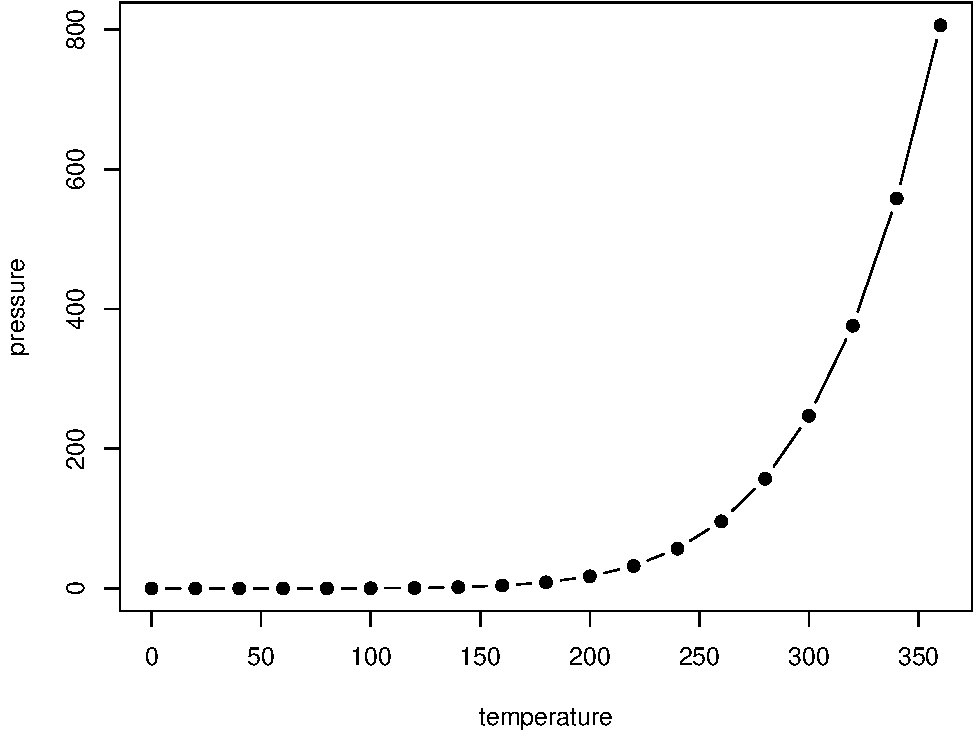
\includegraphics[width=0.8\linewidth]{thesis_files/figure-latex/nice-fig-1} 

}

\caption{Here is a nice figure!}\label{fig:nice-fig}
\end{figure}

Don't miss Table \ref{tab:nice-tab}.

\begin{Shaded}
\begin{Highlighting}[]
\NormalTok{knitr}\SpecialCharTok{::}\FunctionTok{kable}\NormalTok{(}
  \FunctionTok{head}\NormalTok{(pressure, }\DecValTok{10}\NormalTok{), }\AttributeTok{caption =} \StringTok{\textquotesingle{}Here is a nice table!\textquotesingle{}}\NormalTok{,}
  \AttributeTok{booktabs =} \ConstantTok{TRUE}
\NormalTok{)}
\end{Highlighting}
\end{Shaded}

\begin{table}

\caption{\label{tab:nice-tab}Here is a nice table!}
\centering
\begin{tabular}[t]{rr}
\toprule
temperature & pressure\\
\midrule
0 & 0.0002\\
20 & 0.0012\\
40 & 0.0060\\
60 & 0.0300\\
80 & 0.0900\\
\addlinespace
100 & 0.2700\\
120 & 0.7500\\
140 & 1.8500\\
160 & 4.2000\\
180 & 8.8000\\
\bottomrule
\end{tabular}
\end{table}

\hypertarget{parts}{%
\chapter{Parts}\label{parts}}

You can add parts to organize one or more book chapters together. Parts can be inserted at the top of an .Rmd file, before the first-level chapter heading in that same file.

Add a numbered part: \texttt{\#\ (PART)\ Act\ one\ \{-\}} (followed by \texttt{\#\ A\ chapter})

Add an unnumbered part: \texttt{\#\ (PART\textbackslash{}*)\ Act\ one\ \{-\}} (followed by \texttt{\#\ A\ chapter})

Add an appendix as a special kind of un-numbered part: \texttt{\#\ (APPENDIX)\ Other\ stuff\ \{-\}} (followed by \texttt{\#\ A\ chapter}). Chapters in an appendix are prepended with letters instead of numbers.

\hypertarget{footnotes-and-citations}{%
\chapter{Footnotes and citations}\label{footnotes-and-citations}}

\hypertarget{footnotes}{%
\section{Footnotes}\label{footnotes}}

Footnotes are put inside the square brackets after a caret \texttt{\^{}{[}{]}}. Like this one \footnote{This is a footnote.}.

\hypertarget{citations}{%
\section{Citations}\label{citations}}

Reference items in your bibliography file(s) using \texttt{@key}.

For example, we are using the \textbf{bookdown} package (Xie 2021) (check out the last code chunk in index.Rmd to see how this citation key was added) in this sample book, which was built on top of R Markdown and \textbf{knitr} (Xie 2015) (this citation was added manually in an external file book.bib).
Note that the \texttt{.bib} files need to be listed in the index.Rmd with the YAML \texttt{bibliography} key.

The RStudio Visual Markdown Editor can also make it easier to insert citations: \url{https://rstudio.github.io/visual-markdown-editing/\#/citations}

\hypertarget{blocks}{%
\chapter{Blocks}\label{blocks}}

\hypertarget{equations}{%
\section{Equations}\label{equations}}

Here is an equation.

\begin{equation} 
  f\left(k\right) = \binom{n}{k} p^k\left(1-p\right)^{n-k}
  \label{eq:binom}
\end{equation}

You may refer to using \texttt{\textbackslash{}@ref(eq:binom)}, like see Equation \eqref{eq:binom}.

\hypertarget{callout-blocks}{%
\section{Callout blocks}\label{callout-blocks}}

The R Markdown Cookbook provides more help on how to use custom blocks to design your own callouts: \url{https://bookdown.org/yihui/rmarkdown-cookbook/custom-blocks.html}

\hypertarget{sharing-your-book}{%
\chapter{Sharing your book}\label{sharing-your-book}}

\hypertarget{publishing}{%
\section{Publishing}\label{publishing}}

HTML books can be published online, see: \url{https://bookdown.org/yihui/bookdown/publishing.html}

\hypertarget{pages}{%
\section{404 pages}\label{pages}}

By default, users will be directed to a 404 page if they try to access a webpage that cannot be found. If you'd like to customize your 404 page instead of using the default, you may add either a \texttt{\_404.Rmd} or \texttt{\_404.md} file to your project root and use code and/or Markdown syntax.

\hypertarget{metadata-for-sharing}{%
\section{Metadata for sharing}\label{metadata-for-sharing}}

Bookdown HTML books will provide HTML metadata for social sharing on platforms like Twitter, Facebook, and LinkedIn, using information you provide in the \texttt{index.Rmd} YAML. To setup, set the \texttt{url} for your book and the path to your \texttt{cover-image} file. Your book's \texttt{title} and \texttt{description} are also used.

This \texttt{gitbook} uses the same social sharing data across all chapters in your book- all links shared will look the same.

Specify your book's source repository on GitHub using the \texttt{edit} key under the configuration options in the \texttt{\_output.yml} file, which allows users to suggest an edit by linking to a chapter's source file.

Read more about the features of this output format here:

\url{https://pkgs.rstudio.com/bookdown/reference/gitbook.html}

Or use:

\begin{Shaded}
\begin{Highlighting}[]
\NormalTok{?bookdown}\SpecialCharTok{::}\NormalTok{gitbook}
\end{Highlighting}
\end{Shaded}

\cleardoublepage
    \bookmarksetupnext{level=part}
    \phantomsection
    \addcontentsline{toc}{chapter}{References}
    \begin{centering}
    REFERENCES\\
    \vskip 1 \baselineskip
    \end{centering}

\hypertarget{refs}{}
\begin{CSLReferences}{1}{0}
\leavevmode\vadjust pre{\hypertarget{ref-arentze00}{}}%
Arentze, Theo, and Harry Timmermans. 2000. \emph{Albatross: A Learning Based Transportation Oriented Simulation System}. Citeseer.

\leavevmode\vadjust pre{\hypertarget{ref-ben02}{}}%
Ben-Akiva, Moshe, Daniel Mcfadden, Kenneth Train, Joan Walker, Chandra Bhat, Michel Bierlaire, Denis Bolduc, et al. 2002. {``Hybrid Choice Models: Progress and Challenges.''} \emph{Marketing Letters} 13 (3): 163--75. \url{https://doi.org/10.1023/a:1020254301302}.

\leavevmode\vadjust pre{\hypertarget{ref-ben02num2}{}}%
Ben-Akiva, Moshe, Joan Walker, Adriana T. Bernardino, Dinesh A. Gopinath, Taka Morikawa, and Amalia Polydoropoulou. 2002. {``Integration of Choice and Latent Variable Models.''} \emph{In Perpetual Motion}, 431--70. \url{https://doi.org/10.1016/b978-008044044-6/50022-x}.

\leavevmode\vadjust pre{\hypertarget{ref-bhat95}{}}%
Bhat, Chandra R. 1995. {``A Heteroscedastic Extreme Value Model of Intercity Travel Mode Choice.''} \emph{Transportation Research Part B: Methodological} 29 (6): 471--83.

\leavevmode\vadjust pre{\hypertarget{ref-bhat99}{}}%
Bhat, Chandra R, and Frank S Koppelman. 1999. {``Activity-Based Modeling of Travel Demand.''} In \emph{Handbook of Transportation Science}, 35--61. Springer.

\leavevmode\vadjust pre{\hypertarget{ref-bowman01}{}}%
Bowman, J. L, and M. E Ben-Akiva. 2001. {``Activity-Based Disaggregate Travel Demand Model System with Activity Schedules.''} \emph{Transportation Research Part A: Policy and Practice} 35 (1): 1--28. \url{https://doi.org/10.1016/s0965-8564(99)00043-9}.

\leavevmode\vadjust pre{\hypertarget{ref-bowman99}{}}%
Bowman, John L, Mark Bradley, Yoram Shiftan, T Keith Lawton, and Moshe Ben-Akiva. 1999. {``Demonstration of an Activity-Based Model for Portland.''} In \emph{World Transport Research: Selected Proceedings of the 8th World Conference on Transport ResearchWorld Conference on Transport Research Society}. Volume 3.

\leavevmode\vadjust pre{\hypertarget{ref-eluru10}{}}%
Eluru, Naveen, Abdul Pinjari, Ram Pendyala, and Chandra Bhat. 2010. {``An Econometric Multi-Dimensional Choice Model of Activity-Travel Behavior.''} \emph{Transportation Letters} 2 (4): 217--30. \url{https://doi.org/10.3328/tl.2010.02.04.217-230}.

\leavevmode\vadjust pre{\hypertarget{ref-bhat20}{}}%
Goulias, Konstadinos G., Adam Wilkinson Davis, and Chandra R. Bhat. 2020. {``Chapter 5 - Consumer Choice Modeling: The Promises and the Cautions.''} In \emph{Mapping the Travel Behavior Genome}, 63--80. Elsevier.

\leavevmode\vadjust pre{\hypertarget{ref-hasnine21}{}}%
Hasnine, Md Sami, and Khandker Nurul Habib. 2021. {``Tour-Based Mode Choice Modelling as the Core of an Activity-Based Travel Demand Modelling Framework: A Review of State-of-the-Art.''} \emph{Transport Reviews} 41 (1): 5--26. \url{https://doi.org/10.1080/01441647.2020.1780648}.

\leavevmode\vadjust pre{\hypertarget{ref-manski2001}{}}%
Manski, Charles F. 2001. {``Daniel McFadden and the Econometric Analysis of Discrete Choice.''} \emph{The Scandinavian Journal of Economics} 103 (2): 217--29.

\leavevmode\vadjust pre{\hypertarget{ref-mcfadden1973}{}}%
McFadden, Daniel et al. 1973. {``Conditional Logit Analysis of Qualitative Choice Behavior.''}

\leavevmode\vadjust pre{\hypertarget{ref-mcfadden86}{}}%
McFadden, Daniel. 1986. {``The Choice Theory Approach to Market Research.''} \emph{Marketing Science} 5 (4): 275--97.

\leavevmode\vadjust pre{\hypertarget{ref-mcnally2000four}{}}%
McNally, Michael G. 2000. {``The Four Step Model.''} In \emph{Handbook of Transport Modelling}. Emerald Group Publishing Limited.

\leavevmode\vadjust pre{\hypertarget{ref-ortuzar94}{}}%
Ortuzar, J.de D., and L. G.Willumsen. 1994. Wiley.

\leavevmode\vadjust pre{\hypertarget{ref-paulssen14}{}}%
Paulssen, Marcel, Dirk Temme, Akshay Vij, and Joan L. Walker. 2014. {``Values, Attitudes and Travel Behavior: A Hierarchical Latent Variable Mixed Logit Model of Travel Mode Choice.''} \emph{Transportation} 41 (4): 873--88. \url{https://doi.org/10.1007/s11116-013-9504-3}.

\leavevmode\vadjust pre{\hypertarget{ref-pendyala97}{}}%
Pendyala, Ram M, Ryuichi Kitamura, Cynthia Chen, and Eric I Pas. 1997. {``An Activity-Based Microsimulation Analysis of Transportation Control Measures.''} \emph{Transport Policy} 4 (3): 183--92.

\leavevmode\vadjust pre{\hypertarget{ref-pinjari07}{}}%
Pinjari, Abdul Rawoof, Ram M. Pendyala, Chandra R. Bhat, and Paul A. Waddell. 2007. {``Modeling Residential Sorting Effects to Understand the Impact of the Built Environment on Commute Mode Choice.''} \emph{Transportation} 34 (5): 557--73. \url{https://doi.org/10.1007/s11116-007-9127-7}.

\leavevmode\vadjust pre{\hypertarget{ref-vij13}{}}%
Vij, Akshay, André Carrel, and Joan L. Walker. 2013. {``Incorporating the Influence of Latent Modal Preferences on Travel Mode Choice Behavior.''} \emph{Transportation Research Part A: Policy and Practice} 54: 164--78. \url{https://doi.org/10.1016/j.tra.2013.07.008}.

\leavevmode\vadjust pre{\hypertarget{ref-xie2015}{}}%
Xie, Yihui. 2015. \emph{Dynamic Documents with {R} and Knitr}. 2nd ed. Boca Raton, Florida: Chapman; Hall/CRC. \url{http://yihui.org/knitr/}.

\leavevmode\vadjust pre{\hypertarget{ref-R-bookdown}{}}%
---------. 2021. \emph{Bookdown: Authoring Books and Technical Documents with r Markdown}. \url{https://CRAN.R-project.org/package=bookdown}.

\end{CSLReferences}


% Index?

\end{document}
